% LTeX: language=es
\documentclass[a4paper]{article}
\usepackage[utf8]{inputenc}
\usepackage{graphicx}
\usepackage{wrapfig}
\usepackage{xurl}
\PassOptionsToPackage{hyphens}{url}
\usepackage{hyperref}

\usepackage{microtype}

\usepackage{fontspec}

\setmainfont[BoldFont=iosevka-aile-bold.ttf,ItalicFont=iosevka-aile-italic.ttf]{iosevka-aile-regular.ttf}

\renewcommand{\sfdefault}{iosevka-aile-regular}

\setlength{\parindent}{15pt}
\usepackage{parskip}

\usepackage{indentfirst}

\usepackage{ragged2e}

\usepackage{setspace}
\onehalfspacing

\setlength{\parindent}{15pt}

\usepackage{parskip}

\usepackage{indentfirst}
\renewcommand\figurename{Fig.}


\usepackage{fancyhdr}
\pagestyle{fancy}
\fancyhf{}
\fancyhead[LO]{\leftmark}
\fancyhead[RE]{\rightmark}
\fancyhead[RO,LE]{\begin{picture}(0,0) \put(-60.38,0){
\includegraphics[width=20mm]{imgs/title/logo.png}} \end{picture}}
\fancyfoot[LE,RO]{\thepage}
\renewcommand{\footrulewidth}{0.4pt}
\fancyhead[LO]{\vspace{-0.3cm} \leftmark \vspace{0.3cm}}


\title{Toma de decisiones}
\author{Markel Fernandez - Emil Nuñez - Joana Renteria - Nicolas Rodriguez}
\date{Octube 2022 -- Noviembre 2022}

\begin{document}
	\begin{titlepage}
    	\begin{center}
    		\begin{figure}[htb]
    			\begin{center}
    				
\includegraphics[width=4cm]{imgs/title/logo.png}
    			\end{center}
    		\end{figure}
    		
    		\vspace*{0.25in}
    		2DAMi
    		\vspace*{0.3in}
    		
    		\begin{Large}
        		\huge{\textbf{Toma de decisiones del reto intermodular 1}} \\
    		\end{Large}
    		
    		\vspace*{0.4in}
    		\begin{figure}[h!]
        		\centering
        		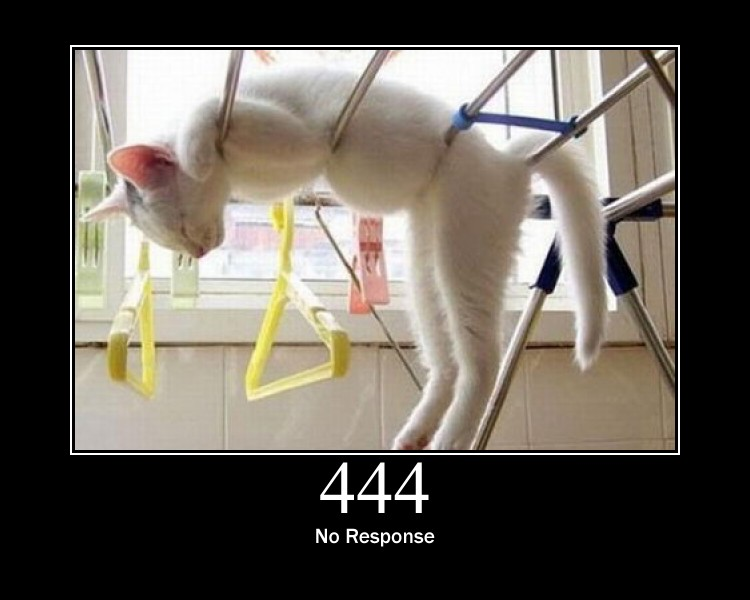
\includegraphics[width=300pt]{imgs/title/portada.jpg}
        		\label{titulo}
    		\end{figure}
    		
    		\begin{large}
				Markel Fernández -- Emil Nuñez -- Joana Renteria -- Nicolás Rodríguez
    		\end{large}
    		
    		\vspace*{0.4in}
    		\rule{90mm}{0.1mm}\\
    		\vspace*{0.1in}
    		\begin{large}
        		Octubre 2022 -- Noviembre 2022\\
    		\end{large}
    	
    	\end{center}
	\end{titlepage}

	\newpage

	\section{Introducción}
		Se nos ha encomendado desarrollar una aplicación que permita a
		sus usuarios \textbf{Iniciar sesión} y \textbf{Registrarse}.
		
		La aplicación se compone de dos partes, el cliente y el servidor. 
		
	\section{2022-10-04}
		\subsection{Decisiones tomadas}
			\begin{itemize}
				\item Prohibido usar nulls
			\end{itemize}
	\section{2022-10-05}
		\subsection{TODO}
			\begin{itemize}
				\item Diagrama de clases
				\item Diagrama de navegación
				\item Documento de diseño
				\item Base de datos
				\item Nomenclatura
				\item Estimación de tiempo -- Planificación
			\end{itemize}
		\subsection{Decisiones tomadas}
			\begin{itemize}
				\item Usar stream de objetos para la comunicación cliente-servidor
					-- UserOrder
			\end{itemize}
	\section{2022-10-06}
		\subsection{TODO}
			\begin{itemize}
				\item Poner el servidor en marcha, faltan configuraciones
				\item Hacer el diagrama de clases
			\end{itemize}
		\subsection{Decisiones tomadas}
			\begin{itemize}
				\item El equipo que vamos a usar para el servidor odoo
			\end{itemize}
	\section{2022-10-07}
		\subsection{TODO}
			\begin{itemize}
				\item Poner el servidor en marcha, faltan configuraciones
				\item Hacer el diagrama de clases
			\end{itemize}
		\subsection{Decisiones tomadas}
			\begin{itemize}
				\item La arquitectura del cliente y del servidor -- 
					Hemos decidido llamar a todo desde los controladores
				\begin{itemize}
					\item Nomenclaturas: camel case, clases con la primera mayuscula, objetos en singular,
						loquesea controller, interfaces -> ables, variables indicativas, metodos autoexplicativos,
						conseguir datos con un get por delante, al acceso a datos le pasamos el objeto,
						el mismo orden de parámetros respecto a la base de datos, comentarios explicando funciones,
						comentarios explicando lambdas
					\item ramas principales: devNombreFuncion
				\end{itemize}
			\end{itemize}
	\section{Nomenclatura}
		\subsection{Variables, Clases y Métodos}
			Vamos a usar camelCase para todo, las clases deberán llevar la primera mayúscula,
			los controladores deberían llamarse NombreController, las factorías
		\subsection{Comentarios}
			Hemos decidido escribir todos los comentarios y javadoc en inglés.
			Como normal general vamos a comentar los métodos y las funciones lambda,
			en caso de que sea necesario, también comentaremos variables.
\end{document}
